%%%%%%%%%%%%%%%%%%%%%%%%%%%%%%%%%%%%%%%%%%%%%%%%%%%%%%%
%% Bachelor's & Master's Thesis Template             %%
%% Copyleft by Artur M. Brodzki & Piotr Woźniak      %%
%% Faculty of Electronics and Information Technology %%
%% Warsaw University of Technology, 2019-2020        %%
%%%%%%%%%%%%%%%%%%%%%%%%%%%%%%%%%%%%%%%%%%%%%%%%%%%%%%%

\documentclass[
    left=2.5cm,         % Sadly, generic margin parameter
    right=2.5cm,        % doesnt't work, as it is
    top=2.5cm,          % superseded by more specific
    bottom=3cm,         % left...bottom parameters.
    bindingoffset=6mm,  % Optional binding offset.
    nohyphenation=false % You may turn off hyphenation, if don't like.
]{eiti/eiti-thesis}

\langpol % Dla języka angielskiego mamy \langeng
\graphicspath{{img/}}             % Katalog z obrazkami.
\addbibresource{bibliografia.bib} % Plik .bib z bibliografią

\begin{document}

%--------------------------------------
% Strona tytułowa
%--------------------------------------
\EngineerThesis % Dla pracy inżynierskiej mamy \EngineerThesis
\instytut{Informatyki}
\kierunek{Informatyka}
\specjalnosc{Inżynieria systemów informatycznych}
\title{
    Wykorzystanie kamery przez aplikacje w systemie Android 
}
\engtitle{ % Tytuł po angielsku do angielskiego streszczenia
    Agnielski tytuł
}
\author{Adamski Maciej}
\album{300184}
\promotor{prof. Przemysław Rokita}
\date{\the\year}
\maketitle

%--------------------------------------
% Streszczenie po polsku
%--------------------------------------
% \cleardoublepage % Zaczynamy od nieparzystej strony
% \streszczenie \lipsum[1-3]
% \slowakluczowe XXX, XXX, XXX

%--------------------------------------
% Streszczenie po angielsku
%--------------------------------------
% \newpage
% \abstract \kant[1-3]
% \keywords XXX, XXX, XXX

%--------------------------------------
% Oświadczenie o autorstwie
%--------------------------------------
%\cleardoublepage  % Zaczynamy od nieparzystej strony
%\pagestyle{plain}
%\makeauthorship

%--------------------------------------
% Spis treści
%--------------------------------------
\cleardoublepage % Zaczynamy od nieparzystej strony
\tableofcontents

%--------------------------------------
% Rozdziały
%--------------------------------------
\cleardoublepage % Zaczynamy od nieparzystej strony
\pagestyle{headings}

\newpage 

\section{Dataset}
\label{section:dataset}
Na potrzeby badań i porównania algorytmów przygotowałem dataset składający się z 80 zdjęć zawierających twarze. 
\par
Źródła zdjęć:

\begin{itemize}
    \item 50 zdjęć wybranych z datasetu \textit{Young and Old Images Dataset} \cite{young_old_dataset}
    \item 30 zdjęć mojego autorstwa
\end{itemize}

Dataset został przygotowany w taki sposób, żeby zawierał zróżnicowane zdjęcia pod wieloma względami, takimi jak: jakość obrazu, oświetlenie, powierzchnia zajmowana przez twarz, kolorystyka, płeć, kolor skóry, częściowe zakrycie twarzy, okulary czy odwrócona w bok głowa. 
Wszystkie 80 zdjęć zostało opisanych przeze mnie na potrzeby badań, w szczególności: obszar twarzy, oczu czy środek źrenic. 
\par
Dodatkowo do badania detekcji źrenic zostanie użyty \textit{MRL Eye Dataset} \cite{mrl_eye_dataset} zawierający zdjęcia oczu wraz z pozycją środka źrenicy.
\newpage

\section{Detekcja twarzy} \label{section:face_detection}

W~przetwarzaniu cyfrowym obrazu stosujemy technikę od ogółu do szczegółu. Przykładowo chcąc uzyskać barwę nadwodzia najpierw musimy wykryć samochód itp. W~pracy dyplomowej by~uzyskać dane dotyczące oczy czy znaczników potrzebujemy najpierw informacji o~tym czy twarz występuje na zdjęciu i~ewentualnie gdzie się ona na~nim znajduje. Dlatego pierwszym etapem przetwarzania na~potrzeby projektu jest detekcja ludzkiej twarzy. Z~dostarczonego obrazu uzyskujemy informację o~jej położeniu, a~w~następnych etapach możemy operować tylko na wycinku zdjęcia. 

\subsection{Algorytmy detekcji twarzy}

Na~potrzeby projektu zostało zaimplementowane użycie pięciu algorytmów, których celem jest wykrycie twarzy na zdjęciu. Krótki opis poszczególnych metod znajduje się w~następnych podrozdziałach.

\subsubsection{Klasyfikator kaskadowy} \label{section:face_casacde_classifier}
\textit{Cascade Classifier} to~jedno z podejść do~zadania klasyfikacji obiektów. Kaskadowość tego rozwiązania przejawia się tym, że składa się on z~łańcucha mniejszych klasyfikatorów. Z~danych wejściowych jednego mogą korzystać następne jako dodatkowe źródło informacji i~użyć je do własnej klasyfikacji. Z~tego powodu kolejne elementy są bardziej zaawansowane i~operują na większym zestawie danych. Dzięki swojej kaskadowej naturze modele takie mogą być lepiej trenowane i~dawać lepsze rezultaty niż klasyfikatory typu monolit.

\vspace{5mm}

Do ładowania i~przetwarzania kaskadowych klasyfikatorów w~projekcie używany jest moduł \textit{CascadeClassifier} \cite{cascade_opencv} biblioteki OpenCV. 

\paragraph{Haar}

Jednym z najbardziej znanych modeli klasyfikacji kaskadowej jest \textit{Haar}, który został opisany po~raz pierwszy w~2001 roku \cite{haar_proceeding}. Może on być używany do~klasyfikacji różnych obiektów, ale~autorzy skupiali się głównie na detekcji twarzy. Algorytm \cite{haar_towards} \cite{haar_pyimage} \cite{OBUKHOV2011517} bazuje na~podzieleniu zdjęcia na~regiony i~wykorzystaniu w~każdym z~nich pięciu cech krawędzi (\hyperref[{fig:haar_features}]{rys.~\ref{fig:haar_features}}). Algorytm porównując jasność pikseli w~białej i~czarnej części stwierdza czy istnieją krawędzie lub linie. Cechy składające się tylko z~dwóch regionów odpowiadają za~wykrycie pionowych i~poziomych krawędzi. Zestaw trzech za~detekcje linii. Natomiast kwadratowa cecha za~zmiany przekątne. W~dzisiejszych czasach Haar nie jest już tak często stosowany jak jeszcze parę lat temu.

\begin{figure}[!h]
    \begin{center}
        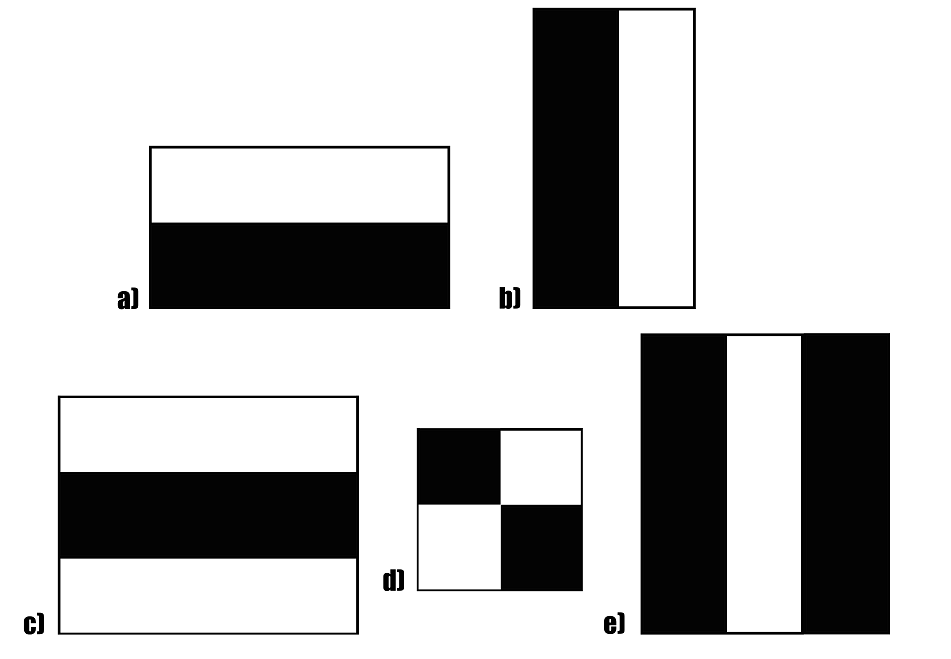
\includegraphics[scale=0.2]{img/face_section/haar_features.png}
        \caption{Cechy krawędzi modelu Haar. Źródło: \cite{haar_towards}}
        \label{fig:haar_features}
    \end{center}
\end{figure}

Na potrzeby pracy dyplomowej wykorzystywany jest model \textit{Haarcascade Frontalface Default} \cite{haar_frontal} autorstwa Rainera Lienharta.



\paragraph{Local binary patterns}
Metoda ta porównuje piksele z~ośmioma swoimi najbliższymi sąsiadami w~ustalonej kolejności. Jeśli jasność głównego piksela jest większa niż porównywanego to~na~odpowiedniej pozycji 8-bitowego ciągu wstawiana jest wartość~1, inaczej~0. Następnie z~uzyskanych w ten sposób liczb tworzony jest histogram używany jako deskryptor cech. Takie dane mogą być użyte do uczenia maszynowego. \cite{comp_haar_lbp}

\par

Jest to metoda cechująca się wysoką szybkością działania i~z~tego powodu stosowana w systemach z~ograniczonymi zasobami sprzętowymi. Niestety kosztem efektywności.

\par

W projekcie stosowany jest model \textit{LBP Cascade Frontalface} \cite{lbp_xml}.


\subsubsection{Histogram zorientowanych gradientów}
Metoda \textit{HOG (Histograms of Oriented Gradients)} \cite{hog_article} została opracowana kilkanaście lat temu przez Navneet Dalal i~Bill Triggs celem detekcji ludzkiego ciała. Aktualnie, mimo upływu lat wciąż jest szeroko wykorzystywana do klasyfikacji obrazów czy wykrywania twarzy.

\par

Uzyskanie histogramu HOG składa się z~kilku etapów. Metoda \cite{hog_wprowadzenie} \cite{learnopencv_HOG} \cite{guide_hog} ta bazuje na~obliczeniu gradientów poziomych i~pionowych. Możliwe jest to~poprzez filtrowanie za pomocą odpowiedniego jądra lub wykorzystując operator Sobela \cite{feature_extraction}. Dla tak wyodrębnionych gradientów oblicza się ich długość i~kierunek (kąt). Następnie dzielimy zdjęcie na~obszary o wielkości $8x8$. Dla każdego regionu tworzymy jednowymiarowy wektor o~9~komórkach, w~których będzie zapisany histogram HOG. Pola wektora odzwierciedlają kierunek gradientu i~odpowiadają kolejnym wielokrotnościom kąta $\measuredangle 20 ^{\circ}$. Wypełniamy go~dodając do~pól odpowiadającym danemu kątowi wartość gradientu kolejnych pikseli. Jeśli kierunek znajduje się pomiędzy dwoma kątami to~wartość dzieli się zależnie od~różnicy między dwiema komórkami. Celem wyeliminowania wpływu jasności i~oświetlenia przeprowadza się normalizację wartości. Gdy obliczy się już histogram dla każdego regionu, łączy się je w~wektor deskryptora cech HOG. Tak uzyskany wektor możemy wykorzystać jako dane uczące algorytmów klasyfikujących. W przypadku metody HOG często wykorzystuje się \textit{maszynę wektorów nośnych (SVM)} \cite{svm_toward_science}.

\vspace{5mm}

Metoda HOG wykorzystywana w~projekcie zaimplementowana jest w bibliotece dlib, która uczona była z~użyciem liniowego SVM.



\subsubsection{Konwolucyjne sieci neuronowe}

\textit{Konwolucyjne sieci neuronowe (CNN)} uczą się jakie cechy obrazu pozwalają sklasyfikować widoczne na~nim obiekty. Za pomocą operacji splotowych, nakładając odpowiednie filtr są wstanie je uwypuklić i~uzyskać istotne informacje. To właśnie w warstwach konwolucyjnych używane są odpowiednie jądra przekształceń. Sieć poprzez trening sama dobiera optymalne filtry oraz ich wartości. Dodatkowo występują warstwy próbkowania (ang. \textit{downsampling} - próbkowanie w dół), których celem jest~zmniejszenie wielkości obrazu przez pominięcie części pikseli. Pomaga to~uprościć sieć, lecz kosztem utraty pewnej ilości informacji. Czasem zamiast pomijać piksele brane są wartości uśredniane lub maksymalne z~pewnego sąsiedztwa. \cite{jak_cnn}

\vspace{5mm}

W bibliotece dlib sieć CNN często jest zestawiona z~metodą \textit{Max-Margin Object Detection (MMMOD)} \cite{mmod}. Służy ona do~optymalizacji i~zwiększenia prędkości detekcji obiektów.

\par

Taka implementacja CNN+MMOD dostępna w dlib stosowana jest w~pracy dyplomowej.



\subsubsection{Głębokie sieci neuronowe}


\textit{Głębokie sieci neuronowe (DNN)} różnią się od~klasycznych tym, że~mają większą liczbę warstw ukrytych. Taki algorytm tworzy plamki o~ustalonej wielkości ze~zdjęć wejściowych, a~następnie przepuszcza je przez kolejne warstwy sieci celem wykrycia pożądanych obiektów. Na wyjściu podaje prawdopodobieństwo okręslające z jaką pewnością na obrazie znajduje się interesujący nas element.

\par

W projekcie wykorzystywany do~tego jest jeden z~modułów biblioteki OpenCV zawierający implementację DNN \cite{opencv_dnn}

\par

Jednym z~modeli dostępnych do~detekcji twarzy przy pomocy głębokich sieci neuronowych są modele \textit{Caffe} (\textit{Convolutional Architecture for Fast Feature Embedding}) \cite{jia2014caffe}. W~projekcie używany jest wzorzec caffe \textit{res10{\_}300x300{\_}ssd{\_}iter{\_}140000{\_}fp16} \cite{caffemodel_res10}.


\subsection{Filtrowanie zwracanych obszarów twarzy}
\label{section:face_detection_filter}

Użyte algorytmy mogą dawać w wyniku błędnie określone obszary twarzy. Z~tego względu zwracana tablica obszarów poddawana jest filtrowaniu.

\par

Proces ten składa się z następujących etapów:

\begin{itemize}
    \item Na początku odrzucane są obszary, których środek znajduje się poza ustalonym pionowym obszarem (przyjęty został przedział [0.25, 0.75] szerokości). Wynika to~z~założeń, że~osoba używająca urządzenie mobilne korzysta z~niego patrząc na~wprost, a~nie z~boku. Natomiast odchylenie od pionu to indywidualne preferencje - dlatego nie jest określony poziomy obszaru. (\hyperref[{fig:face_boundary}]{rys.~\ref{fig:face_boundary}})

    \begin{figure}[!h]
        \begin{center}
            \subfigure[Przed filtrowaniem zależnym od położenia]{\label{fig:face_boundary_before}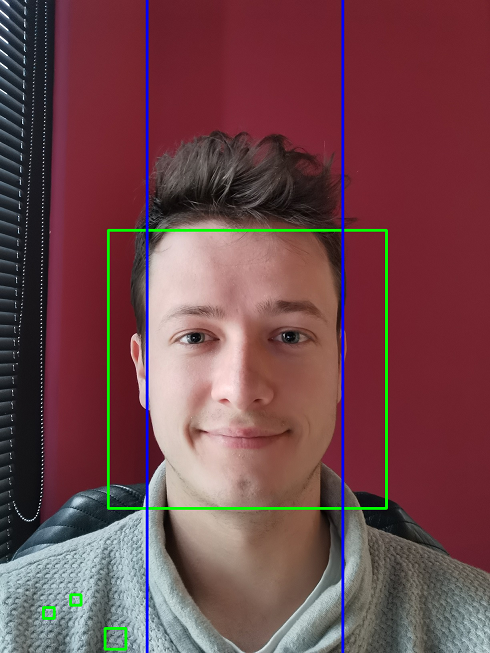
\includegraphics[scale=0.3]{img/face_section/face_filter_boundary_1.png}}
            \hspace{8mm}
            \subfigure[Po filtrowaniu]{\label{fig:face_boundary_after}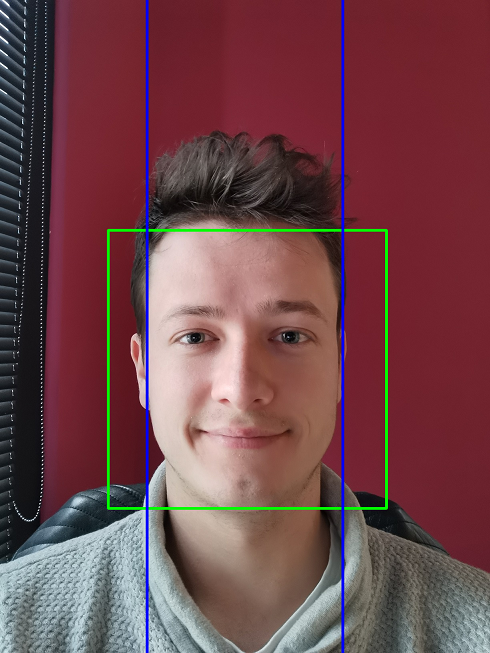
\includegraphics[scale=0.3]{img/face_section/face_filter_boundary_2.png}}
        \end{center}
        \caption{Działanie pierwszego etapu filtrowania detekcji twarzy w oparciu o jej położenie na zdjęciu.}
        \label{fig:face_boundary}
    \end{figure}
    
    \item Kolejnym etapem jest odrzucenie tych detekcji, które wychodzą zbyt daleko poza zdjęcie. Jeśli którykolwiek z~boków prostokąta wystaje pionowo/poziomo o~odległość większą niż $10\%$ odpowiednio wysokości/szerokości to zostaje odrzucony (\hyperref[{fig:face_out}]{rys.~\ref{fig:face_out}}).
    
    \begin{figure}[!h]
        \begin{center}
            \subfigure[Przed filtrowaniem zależnym od wystawania poza obraz]{\label{fig:face_out_before}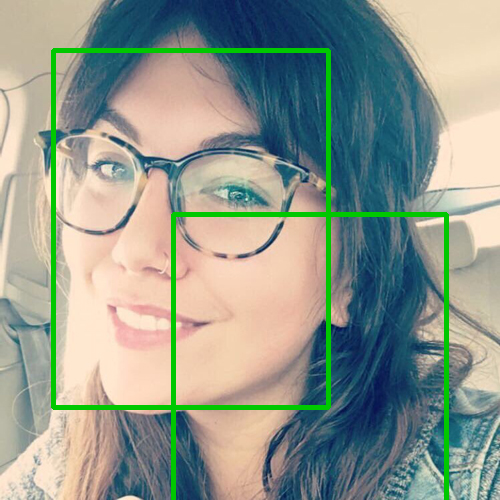
\includegraphics[scale=0.25]{img/face_section/face_filter_out_before.png}}
            \hspace{8mm}
            \subfigure[Po filtrowaniu]{\label{fig:face_out_after}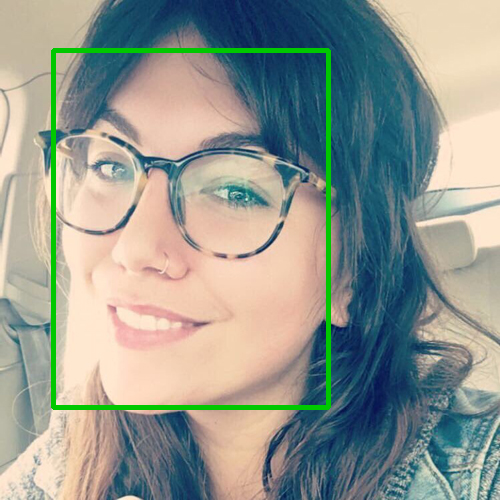
\includegraphics[scale=0.25]{img/face_section/face_filter_out_after.png}}
        \end{center}
        \caption{Działanie drugiego etapu filtrowania detekcji twarzy w oparciu o odległość wykrytego obszaru poza zdjęciem.}
        \label{fig:face_out}
    \end{figure}
    
    \item Z~pozostałych obszarów wybierany jest ten, który zajmuje największą powierzchnię. Taki wybór umotywowany jest własnymi obserwacjami autora na temat zachowania się algorytmów detekcji twarzy oraz tym, że~głowa użytkownika telefonu na obrazie z kamery przedniej zajmuje większą część płaszczyzny, ponieważ korzystając z~urządzenia nie trzymamy go bardzo daleko od siebie. (\hyperref[{fig:face_size}]{rys.~\ref{fig:face_size}})
    
    \begin{figure}[!h]
        \begin{center}
            \subfigure[Przed filtrowaniem zależnym od wielkości]{\label{fig:face_size_before}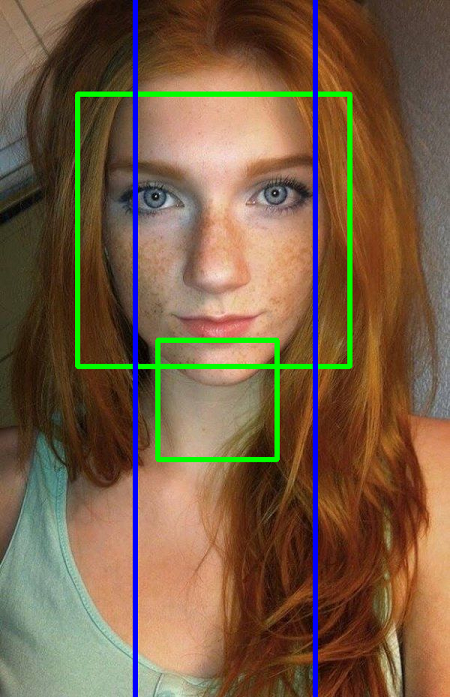
\includegraphics[scale=0.3]{img/face_section/face_filter_size_1.png}}
            \hspace{8mm}
            \subfigure[Po filtrowaniu]{\label{fig:face_size_after}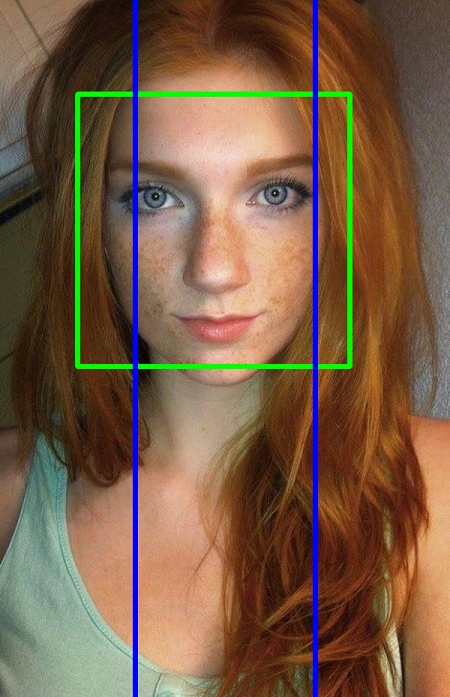
\includegraphics[scale=0.3]{img/face_section/face_filter_size_2.png}}
        \end{center}
        \caption{Działanie ostatniego etapu filtrowania detekcji twarzy w oparciu o wielkość wykrytego obszaru. Źródło zdj.: \cite{readheadPortrait1}}
        \label{fig:face_size}
    \end{figure}
    
    
    
\end{itemize}
\newpage

\section{Detekcja oczu} \label{section:eye_detection}

W tej pracy dyplomowej dużą role odgrywają oczy i ich wpływ na sterowanie aplikacją. Z tego powodu musiała zostać określona i zaimplementowana skuteczna metoda ich detekcji.



\subsection{Algorytmy detekcji oczu}

Na potrzeby tego etapu zostały zastosowane dwie metody opierające się na algorytmach opisanych wcześniej - klasyfikatory kaskadowe oraz facemarki.

\subsubsection{Klasyfikator kaskadowy Haar}

Metody detekcji oparte na klasyfikatorach kaskadowych zostały opisane w rozdz. \hyperref[{section:face_casacde_classifier}]{\textit{\ref{section:face_casacde_classifier}}}. Do detekcji oczu z użyciem tego algorytmu zostanie wykorzystany model autorstwa Shameem Hameed \cite{eye_haar_model}.

\subsubsection{Facemarki}

Opisane w rozdz. \hyperref[section:landmarks]{\ref{section:landmarks}} facemarki nanoszą punkty charakterystyczne na obraz twarzy. Znajdują się one m.in. wokół oczu. Fakt ten można wykorzystać do detekcji ich obszaru. Celem uzyskania takiego efektu należy wyznaczyć prostokąt, który będzie otaczał wszystkie sześć facemarków danego oka. \cite{detect_eye_facemarks}
\par
Przykład takiego działania widoczny jest na rysunku \ref{fig:facemarki_to_detect_eyes}.

\begin{figure}[!h]
    \begin{center}
        \subfigure[Facemarki wokół oka]{\label{fig:facemarki_to_detect_eyes_no_rect}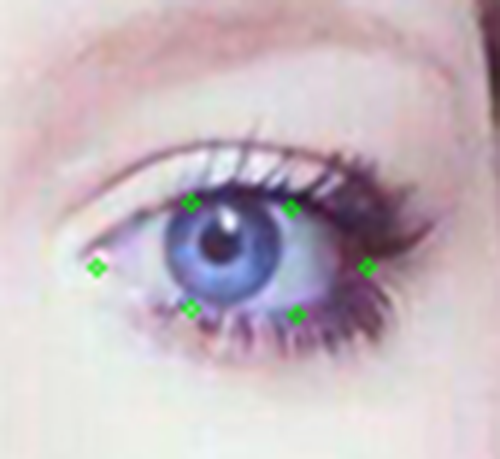
\includegraphics[scale=0.25]{img/eye_section/eye_facemarks.png}}
        \hspace{8mm}
        \subfigure[Naniesiony prostokąt otaczający facemarki wokół oka]{\label{fig:facemarki_to_detect_eyes_rect}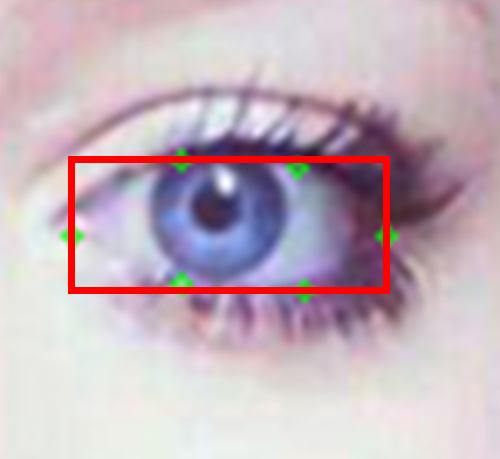
\includegraphics[scale=0.25]{img/eye_section/eye_facemarks_rect.png}}
    \end{center}
    \caption{Wykorzystanie facemarków do detekcji obszaru oczu}
    \label{fig:facemarki_to_detect_eyes}
\end{figure}

Wykorzystywany jest tu też wskaźnik \textit{EAR} (patrz rozdz. \hyperref[{section:EARsection}]{\textit{\ref{section:EARsection}. EAR - Eye Aspect Ratio}}) do wykrycia czy oko jest zamknięte czy otwarte.
\par
Skuteczność tej metody zależy od dokładności algorytmu odwzorowującego facemarki. Ewentualne niedoskonałości można niwelować zwiększając wielkość prostokąta o pewną tolerancję. Taki współczynnik w projekcie został testowo ustalony, a wyniki i wartości parametrów opisane w rozdz. \hyperref[{section:facemark_eye_size}]{\textit{\ref{section:facemark_eye_size}}}.



\subsection{Filtrowanie wyników metody Haar}

Ze względu, że algorytmu Haar może zwracać większą ilość prawdopodobnych obszarów, w których spodziewa się on wykryć pożądany obiekt, wprowadziłem filtrowanie wyników detekcji oczu. \\
Algorytm filtrowania składa się z dwóch etapów:

\begin{itemize}
    \item Podzielenie wykrytych obszarów na dwie grupy - na lewą i prawą stronę twarzy
    \item W obu grupach wybranie największego obszaru
\end{itemize}


Dodatkowo pozwoliło to na łatwe zidentyfikowanie który obszar to które oko i ich posortowanie.
\par
Przykładowy rezultat takiego filtrowania pokazany jest na \hyperref[{fig:eye_filter}]{\textit{rysunku \ref{fig:eye_filter}}}. 


\begin{figure}[!h]
    \begin{center}
        \subfigure[Przed filtrowaniem]{\label{fig:eye_filter_before}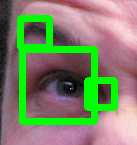
\includegraphics[scale=1.0]{img/eye_section/eye_filter_before.png}}
        \hspace{8mm}
        \subfigure[Po filtrowaniu]{\label{fig:eye_filter_after}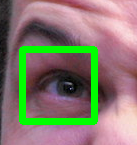
\includegraphics[scale=1.0]{img/eye_section/eye_filter_after.png}}
    \end{center}
    \caption{Efekt filtrowania obszarów detekcji oczu}
    \label{fig:eye_filter}
\end{figure}

\subsection{Obcięcie obszaru detekcji dla metody Haar}

Dla metody opartej na Haar zdecydowałem się dodatkowo zawęzić płaszczyznę przeszukiwań na niecałą twarz, celem uzyskania wyników lepszych niż bez takiego zmniejszenia. 
\par
Ustalenie jaki obszar da najlepszy rezultat odbyło się przez testowe sprawdzanie kombinacji trzech parametrów oznaczających jaka część wykrytej twarzy zostaje obcięta z poszczególnej strony. Mogą one przyjmować wartości w następujących przedziałach:

\begin{itemize}
    \item Góra: $[0.0,$ $0.02]$
    \item Dół: $[0.2,$ $0.6]$
    \item Boki: $[0.0,$ $0.02]$
\end{itemize}

Każdy parametr mógł osiągać wartości będące wielokrotnością $0.05$ w poszczególnych przedziałach.

\par

Ze względu na dużą ilość kombinacji ($225$) nie zostaną podane wyniki, a jedynie wybrana najlepsza kombinacja:
\begin{itemize}
    \item Góra: $0.05$
    \item Dół: $0.3$
    \item Boki: $0.0$
\end{itemize}

Algorytm Haar uzyskał lepszą skuteczność detekcji wykorzystując dodatkowe obcięcie niż bez niego:

\begin{table}[!h]

\centering
\caption{Skuteczność algorytmu detekcji oczu Haar z dodatkowym obcięciem i bez}
\label{tab:eye_haar_crop_result}
\resizebox{\textwidth}{!}{%
\begin{tabular}{|c|c|c|c|c|c|c|}
\hline
 &
  \textbf{\begin{tabular}[c]{@{}c@{}}Prawidłowe\\ detekcje\end{tabular}} &
  \textbf{\begin{tabular}[c]{@{}c@{}}Perfekcyjne\\ detekcje\end{tabular}} &
  \textbf{\begin{tabular}[c]{@{}c@{}}Częściowo\\ dobre\\ detekcje\end{tabular}} &
  \textbf{\begin{tabular}[c]{@{}c@{}}Złe\\ detekcje\end{tabular}} &
  \textbf{\begin{tabular}[c]{@{}c@{}}Niewykryte\\  oczy otwarte\end{tabular}}  &
 \textbf{\begin{tabular}[c]{@{}c@{}}Niewykryte\\  oczy zamknięte \end{tabular}} \\ \hline \hline
\textbf{Haar bez obcięcia} &
  124 &
  85 &
  39 &
  34 &
  8 &
  32  \\ \hline

\textbf{Haar z obcięciem} &
  133 &
  95 &
  38 &
  23 &
  9 &
  11  \\ \hline
  
  \hline
\end{tabular}%
}
\end{table}

Przykład takiego obcięcia z wybranymi parametrami widoczny jest na \hyperref[{fig:eye_crop}]{\textit{rysunku \ref{fig:eye_crop}}}.

\begin{figure}[!h]
    \begin{center}
        \subfigure[Wykryty obszar twarzy]{\label{fig:eye_crop_before}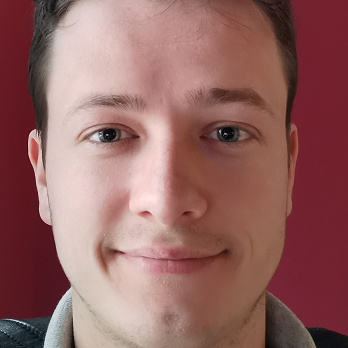
\includegraphics[scale=0.6]{img/eye_section/eye_cropped_face.png}}
        \hspace{8mm}
        \subfigure[Obszar po obcięciu]{\label{fig:eye_crop_after}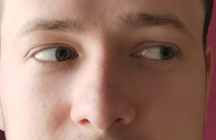
\includegraphics[scale=0.6]{img/eye_section/eye_cropped_eyes.png}}
    \end{center}
    \caption{Obcięcie obszaru detekcji oczu zgodnie z dobranymi wcześniej parametrami}
    \label{fig:eye_crop}
\end{figure}

Wprowadzenie takiej modyfikacji pozwoliło odrzucić część błędnie ustalanych obszarów, szczególnie w dolnej części twarzy. Przykład poprawionej detekcji oczu dzięki temu zabiegowi widoczny jest na rysunku \ref{fig:eye_detect_crop}

\begin{figure}[!h]
    \begin{center}
        \subfigure[Wykrywanie oczu bez dodatkowego obcięcia obszaru]{\label{fig:eye_detect_crop_before}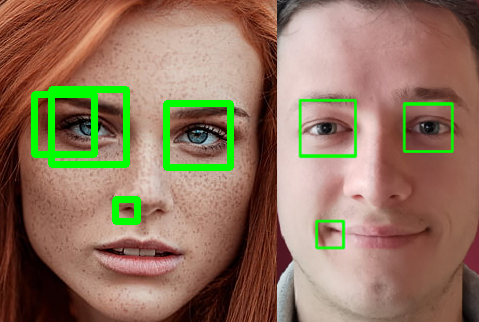
\includegraphics[scale=0.45]{img/eye_section/eye_detect_before_crop_1.png}}
        \hspace{8mm}
        \subfigure[Wykrywanie oczu z dodatkowym obcięciem obszaru]{\label{fig:eye_detect_crop_after}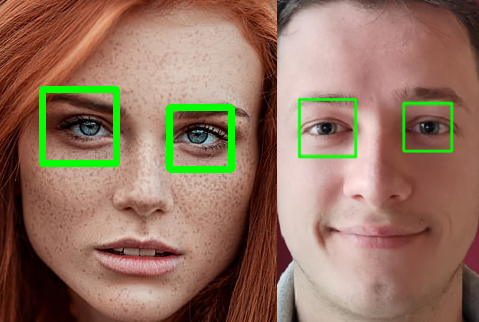
\includegraphics[scale=0.45]{img/eye_section/eye_detect_after_crop_1.png}}
    \end{center}
    \caption{Odrzucenie błędnych rezultatów detekcji oczu po dodatkowym obcięciu obszaru. Źródło pierwszego zdj.:\cite{readheadPortrait2}}
    \label{fig:eye_detect_crop}
\end{figure}


\subsection{Dostosowanie wielkości obszaru facemarków oczu} \label{section:facemark_eye_size}

Dla metody opartej o punkty charakterystyczne twarzy zdecydowałem się dodać pewną tolerancję do obszaru wynikającego jedynie z połączenia tych punktów.
\par
Ustalenie jakie zwiększenie zwracanego regionu da najlepsze rezultaty detekcji oczu odbyło się przez testowe sprawdzenie kombinacji trzech parametrów, które oznaczały wielkość tolerancji z danej strony. W teści przyjmowały one następujące wartości

\begin{itemize}
    \item Góra: z przedziału [0.0, 1.0], będące wielokrotnością $0.1$
    \item Dół: z przedziału [0.0, 1.0], będące wielokrotnością $0.1$
    \item Boki: z przedziału [0.0, 0.5], będące wielokrotnością $0.05$
\end{itemize}

\par

Ze względu na dużą ilość kombinacji ($1331$) nie zostaną podane wyniki, a jedynie wybrana najlepsza kombinacja:
\begin{itemize}
    \item Góra: $0.7$
    \item Dół: $0.5$
    \item Boki: $0.2$
\end{itemize}


\begin{table}[!h]
\label{tab:eye_facemark_size_result}
\centering
\caption{Skuteczność algorytmu detekcji oczu wykorzystując facemarki z dodatkowym zwiększeniem obszaru i bez}
\resizebox{\textwidth}{!}{%
\begin{tabular}{|c|c|c|c|c|c|c|}
\hline
 &
  \textbf{\begin{tabular}[c]{@{}c@{}}Prawidłowe\\ detekcje\end{tabular}} &
  \textbf{\begin{tabular}[c]{@{}c@{}}Perfekcyjne\\ detekcje\end{tabular}} &
  \textbf{\begin{tabular}[c]{@{}c@{}}Częściowo\\ dobre\\ detekcje\end{tabular}} &
  \textbf{\begin{tabular}[c]{@{}c@{}}Złe\\ detekcje\end{tabular}} &
  \textbf{\begin{tabular}[c]{@{}c@{}}Niewykryte\\  oczy otwarte\end{tabular}}  &
 \textbf{\begin{tabular}[c]{@{}c@{}}Niewykryte\\  oczy zamknięte \end{tabular}} \\ \hline \hline
\textbf{\begin{tabular}[c]{@{}c@{}}Facemarki oczu \\ bez zwiększenia obszaru\end{tabular}} &
  142 &
  17 &
  125 &
  14 &
  6 &
  6  \\ \hline

\textbf{\begin{tabular}[c]{@{}c@{}}Facemarki oczu \\ ze zwiększeniem obszaru\end{tabular}} &
  144 &
  142 &
  2 &
  12 &
  6 &
  6  \\ \hline
  
  \hline
\end{tabular}%
}
\end{table}

Zmiany wielkości zwracanego obszaru oczu nie zwiększył znacząco liczby dobrych detekcji. Natomiast największy zysk widoczny jest w perfekcyjnych detekcjach. Dzięki takiemu dostosowaniu udało się osiągnąć prawie $100\%$ wskaźnik perfekcyjnych względem prawidłowych detekcji. Pozwoli to uzyskać lepiej wykryty obszar oczu, co może mieć przełożenie na skuteczność detekcji źrenic.
\newpage

\section{Detekcja źrenic}

W pracy dyplomowej występuje sterowanie aplikacją za pomocą ruch gałek ocznych, w~szczególności analizując położenie źrenic. Mając wykryty obszar oczu (patrz rozdz.~\hyperref[{section:eye_detection}]{\textit{\ref{section:eye_detection}}}) metodami klasycznymi przetwarzania obrazów określane położenie środka źrenicy.

\par

W projekcie zaimplementowane zostały trzy algorytmy do testów i~wybrany jeden, który dawał najlepsze rezultaty.

\subsection{Algorytmy detekcji źrenic}

\subsubsection{Algorytm CDF (Cumulative Distribution Function)}
Algorytm zaimplementowany na podstawie dwóch artykułów o~detekcji źrenic~\cite{IMECSPupilCDFAnalysis}~\cite{EyePupilWebCam}. Opiera się w~głównej mierze na progowaniu za pomocą dystrybuanty. Następnie analizuje najciemniejszy obszar wyznaczany jest środek źrenicy.

\iffalse
\begin{figure}[!h]
    \begin{center}
        \subfigure[Oko skierowane w~prawo]{\label{fig:pupil_cdf_left}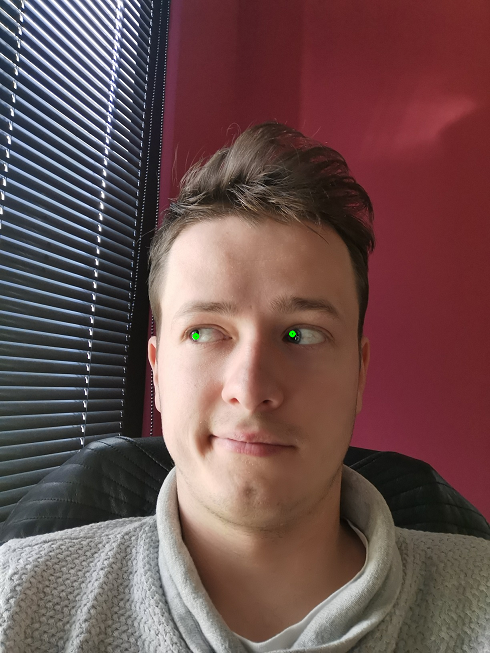
\includegraphics[scale=0.3]{img/pupil_section/pupil_2eyes_left_1.png}}
        \hspace{3mm}
        \subfigure[Oko skierowane na wprost]{\label{fig:pupil_cdf_center}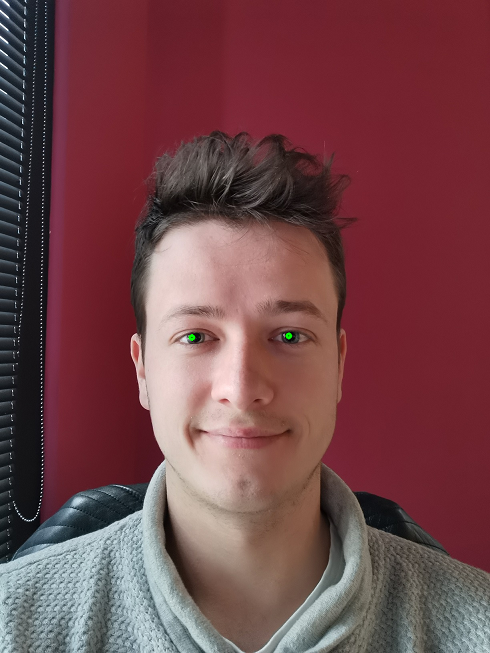
\includegraphics[scale=0.3]{img/pupil_section/pupil_2eyes_center_1.png}}
        \hspace{3mm}
        \subfigure[Oko skierowane w~lewo]{\label{fig:pupil_cdf_right}
\includegraphics[scale=0.3]{img/pupil_section/pupil_2eyes_right_1.png}}
    \end{center}
    \caption{Rezultat wykrywania źrenic metodą CDF}
    \label{fig:cdf_results}
\end{figure}
\fi

\paragraph{Kroki algorytmu}

\begin{itemize}
    \item Za pomocą progowania z~użyciem dystrybuanty tworzony jest obraz binarny.\\
    \begin{align}
        CDF(r) = \sum_{w=0}^{r} p(w)
    \end{align}
    
    Gdzie \textit{p(w)} to prawdopodobieństwo znalezienia punktu o~jasności równej \textit{w} - określone przy pomocy dystrybuanty.
    
    \begin{align}
        I`(x, y) = 
        \begin{cases}
            255, &  CDF(I(x, y)) < \textit{a}\\
            0,   &  wpp
        \end{cases}
    \end{align} 
    
    Gdzie \textit{I} to jasność piksela, natomiast \textit{a} to ustalony próg

    \item Na uzyskany obraz binarny nakładana jest operacja morfologiczna erozji (filtr minimalny), celem usunięcia pojedynczych ciemnych pikseli
    
    \item Następnie znajdowany jest najciemniejszy piksel na oryginalnym obrazie wśród tych, które mają wartość~255 (są białe) na obrazie binarnym
    
    \item Obliczana jest średnia jasność pikseli w~kwadracie~10x10 wokół wybranego najciemniejszego punktu
    
    \item Nakładana jest erozja na obszarze~15x15 wokół wybranego punktu
    
    \item Na tym obszarze stosowane jest progowanie na podstawie wartości
    
    \begin{align}
        I`(x, y) = 
        \begin{cases}
            255, &  I(x, y) < I_{AVG}\\
            0,   &  wp.p.
        \end{cases}
    \end{align}
    
    Gdzie \textit{$I_{AVG}$} to średnia jasność obszaru obliczona wcześniej
    
    \item Szukanym punktem źrenicy jest środek ciężkości białych punktów na uzyskanym binarnym obrazie

\end{itemize}

\iffalse
\begin{figure}[!h]
    \begin{center}
        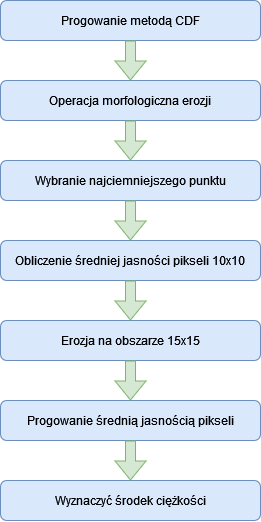
\includegraphics[scale=0.35]{img/pupil_section/CDF_Diagram.png}
        \caption{Kroki algorytmu metodą CDF}
        \label{fig:cdf_diagram}
    \end{center}
\end{figure}
\fi

\paragraph{Wynik kolejnych kroków algorytmu}
Na \hyperref[{fig:cdf_steps}]{\textit{rys.~\ref{fig:cdf_steps}}} przedstawiony jest rezultat kolejnych etapów wykrywania źrenic przy pomocy metody \textit{CDF} na przykładowym zdjęciu oka.

\begin{figure}[!h]
    \begin{center}
        \subfigure[Obszar oka w~skali szarości]{\label{fig:cdf_gray}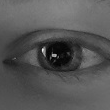
\includegraphics[scale=0.50]{img/pupil_section/CDF_steps/CDF_gray_eye.png}}
        \hspace{8mm}
        \subfigure[Wynik progowania CDF]{\label{fig:cdf_binary}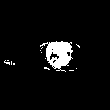
\includegraphics[scale=0.50]{img/pupil_section/CDF_steps/CDF_binary_eye_after_CDF.png}}
        \hspace{8mm}
        \subfigure[Wynik erozji]{\label{fig:cdf_erode}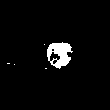
\includegraphics[scale=0.50]{img/pupil_section/CDF_steps/CDF_binary_eye_after_erode.png}}
        
        \hfill
        
        \subfigure[Najciemniejszy punkt]{\label{fig:cdf_darkest}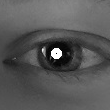
\includegraphics[scale=0.50]{img/pupil_section/CDF_steps/CDF_darkest_pixel.png}}
        \hspace{8mm}
        \subfigure[Obszar 10x10, w~którym obliczana jest średnia jasność]{\label{fig:cdf_avgIntens}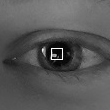
\includegraphics[scale=0.50]{img/pupil_section/CDF_steps/CDF_avgIntensity_region.png}}
        \hspace{8mm}
        \subfigure[Wynik erozji]{\label{fig:cdf_eroded}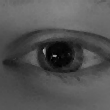
\includegraphics[scale=0.50]{img/pupil_section/CDF_steps/cdf_eroded_eye.png}}
        
        \hfill
        
        \subfigure[Obszar 15x15, który poddawany jest progowaniu]{\label{fig:cdf_pmi}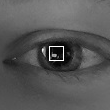
\includegraphics[scale=0.50]{img/pupil_section/CDF_steps/CDF_pmi.png}}
        \hspace{8mm}
        \subfigure[Progowanie średnią jasnością pikseli]{\label{fig:cdf_threshold}
\includegraphics[scale=3.65]{img/pupil_section/CDF_steps/CDF_threshold_pmi.png}}
        \hspace{8mm}
         \subfigure[Wykryte położenie źrenicy]{\label{fig:cdf_pupil_detected}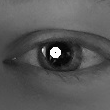
\includegraphics[scale=0.50]{img/pupil_section/CDF_steps/CDF_pupil_detected.png}}

        
    \end{center}
    \caption{Kolejne etapy wykrywania źrenic metodą CDF}
    \label{fig:cdf_steps}
\end{figure}









\subsubsection{Algorytm PF (Projection Function)}

Algorytm po raz pierwszy opisany w~artykule zatytułowanym \textit{Projection Functions for Eye Detection} \cite{projection_function} z~2004 roku. Jest oparty na rzutowaniu jasności pikseli na składowe poziome i~pionowe. Do obliczenia tych wartości wykorzystuje się funkcje projekcji, która może przyjmować różne postaci - z~czego trzy zostały opisane w~tej pracy dyplomowej. Największe różnice wartości oznaczają szybkie zmiany jasności, które mogą być konturami oka.~\cite{EyePupilWebCam}

\paragraph{Funkcja projekcji}

Funkcja projekcji służąca do rzutowania jasności rzędów i~kolumn może przyjmować różne formy. Najczęściej stosowana jest funkcja całkowa, jednak ze względu na swoje niedociągnięcia i~kłopoty z~wykrywaniem wariancji powstały także inne algorytmy. Trzy różne funkcje opisane są poniżej.

\subparagraph{Funkcja całkowa} Wylicza się za jej pomocą średnią jasność pikseli w~danym rzędzie lub kolumnie. w~teorii jest to całka:
\begin{align}
    {IPF_h}(y) = \frac{1}{{x_b}-{x_a}}\int_{x_a}^{x_b} I(x,y) \, \mathrm{d}x
\end{align}
\begin{align}
    {IPF_v}(x) = \frac{1}{{y_b}-{y_a}}\int_{y_a}^{y_b} I(x,y) \, \mathrm{d}y
\end{align}

Ale w~praktyce degeneruje się do funkcji sumy:

\begin{align}
    {IPF_h}(y)=\frac{1}{{x_b}-{x_a}}\sum_{x={x_a}}^{{x_b}} I(x,y)
\end{align}
\begin{align}
    {IPF_v}(x)=\frac{1}{{y_b}-{y_a}}\sum_{y={y_a}}^{{y_b}} I(x,y)
\end{align}

\subparagraph{Funkcja wariancji} Średnia różnica między jasnością danego piksela, a~wyliczonego \textit{IPF} danego rzędu lub kolumny

\begin{align}
    {VPF_h}(y)=\frac{1}{{x_b}-{x_a}}\sum_{x={x_a}}^{{x_b}} (I(x,y) - {IPF_h(y)})
\end{align}
\begin{align}
    {VPF_v}(x)=\frac{1}{{y_b}-{y_a}}\sum_{y={y_a}}^{{y_b}} (I(x,y) - {IPF_v(x)})
\end{align}

Chociaż we wskazanym wyżej artykule funkcja ta występuje w~przedstawionej formie to spotykane są również postacie z~różnicą kwadratową oraz z~pierwiastkami z~obliczonej wartości. 

\subparagraph{Funkcja ogólna} Parametryzowana suma wyliczonych wartości \textit{IPF} i~\textit{VPF}.

\begin{align}
    {GPF_h}(y)=(1-\alpha) * {IPF_h(y)} + \alpha * {VPF_h(y)}
\end{align}
\begin{align}
    {GPF_v}(x)=(1-\alpha) * {IPF_v(x)} + \alpha * {VPF_v(x)} 
\end{align}

Autorzy tej metody zalecają parametr $\alpha = 0.6$ jako dający najlepsze rezultaty.

\paragraph{Kroki algorytmu}

\begin{itemize}
    \item Dla każdego rzędu i~kolumny obliczana jest wartość funkcji projekcji
    \item Dla wyliczonych funkcji projekcji określana jest wartość pochodnej w~każdym rzędzie i~kolumnie
    \item Wybierane są dwa ekstrema dla poziomego i~pionowego wymiaru
    \item Przecięcie wybranych kolumn i~rzędów tworzy prostokąt, którego śreodek jest poszukiwany punkt na źrenicy 
\end{itemize}

\paragraph{Wynik kolejnych kroków algorytmu}
Na \hyperref[{fig:pf_steps}]{\textit{rys.~\ref{fig:pf_steps}}} przedstawiony jest rezultat kolejnych etapów wykrywania źrenic przy pomocy metody \textit{PF} na przykładowym zdjęciu oka.

\begin{figure}[!h]
    \begin{center}
        \subfigure[Obszar oka w~skali szarości]{\label{fig:pf_gray_eye}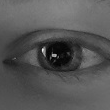
\includegraphics[scale=0.50]{img/pupil_section/PF_steps/PF_gray_eye.png}}
        \hspace{8mm}
        \subfigure[Pionowe wartości projekcji]{\label{fig:pf_x_projection}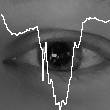
\includegraphics[scale=0.50]{img/pupil_section/PF_steps/PF_x_projection.png}}
        \hspace{8mm}
        \subfigure[Poziome wartości projekcji]{\label{fig:pf_y_projection}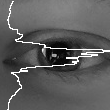
\includegraphics[scale=0.50]{img/pupil_section/PF_steps/PF_y_projection.png}}
        
        \hfill
        
        \subfigure[Pionowe wartości pochodnej]{\label{fig:pf_x_derviatives}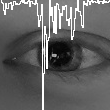
\includegraphics[scale=0.5]{img/pupil_section/PF_steps/PF_x_derivaties.png}}
        \hspace{8mm}
        \subfigure[Poziome wartości pochodnej]{\label{fig:pf_y_derviatives}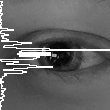
\includegraphics[scale=0.5]{img/pupil_section/PF_steps/PF_y_derivatives.png}}
        \hspace{8mm}
        \subfigure[Pionowe ekstrema]{\label{fig:pf_x_extremum}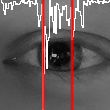
\includegraphics[scale=0.50]{img/pupil_section/PF_steps/PF_x_extremum.png}}
        
        \hfill
        
        \subfigure[Poziome ekstrema]{\label{fig:pf_y_extemum}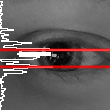
\includegraphics[scale=0.5]{img/pupil_section/PF_steps/PF_y_extremum.png}}
        \hspace{8mm}
        \subfigure[Środek wybranego obszaru]{\label{fig:pf_lines_intersection}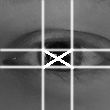
\includegraphics[scale=0.65]{img/pupil_section/PF_steps/PF_lines_intersection.png}}
        \hspace{8mm}
        \subfigure[Wykryte położenie źrenicy]{\label{fig:pf_pupil_detected}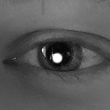
\includegraphics[scale=0.50]{img/pupil_section/PF_steps/PF_pupil_detected.png}}
        
    \end{center}
    \caption{Kolejne etapy wykrywania źrenic metodą PF}
    \label{fig:pf_steps}
\end{figure}






\subsubsection{Algorytm EA (Edge Analysis)}

Algorytm detekcji źrenic \cite{EyePupilWebCam} opierający się na wykryciu i~analizie krawędzi. w~teorii krawędzie najbardziej pionowe i~poziome na zdjęciu powinny należeć do tęczówki i~źrenicy.

\paragraph{Kroki algorytmu}

\begin{itemize}
    \item Dla obszaru oka w~skali szarości nakładany jest filtr rozmywający, np. Gaussa. Pozwala to pozbyć się drobnych szumów i~wygładzić obraz.
    \item Wykrywane są krawędzie i~tworzony obraz binarny. Można zastosować np. algorytm Canny, który jest jedną z~najpopularniejszych metod detekcji krawędzi
    \item Wybierane są dwa rzędy i~dwie kolumny z~największą liczbą punktów o~wartości~255 (białe piksele na obrazie binarnym)
    \item Przecięcie wybranych rzędów i~kolumn tworzy prostokąt, którego środek jest poszukiwany punkt na źrenicy
\end{itemize}

\paragraph{Wynik kolejnych kroków algorytmu}
Na \hyperref[{fig:ea_steps}]{\textit{rys.~\ref{fig:ea_steps}}} przedstawiony jest rezultat kolejnych etapów wykrywania źrenic przy pomocy metody \textit{EA} na przykładowym zdjęciu oka.

\begin{figure}[!h]
    \begin{center}
        \subfigure[Obszar oka w~skali szarości]{\label{fig:ea_gray_eye}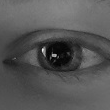
\includegraphics[scale=0.50]{img/pupil_section/EA_steps/EA_gray_eye.png}}
        \hspace{8mm}
        \subfigure[Rozmycie filtrem Gaussa]{\label{fig:ea_gaussian}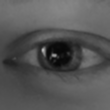
\includegraphics[scale=0.50]{img/pupil_section/EA_steps/EA_gaussian.png}}
        \hspace{8mm}
        \subfigure[Detekcja krawędzi metodą Canny]{\label{fig:ea_canny}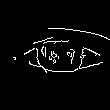
\includegraphics[scale=0.50]{img/pupil_section/EA_steps/EA_canny.png}}
        
        \hfill
        
        \subfigure[Najliczniejsze rzędy i~kolumny]{\label{fig:ea_canny_lines}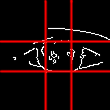
\includegraphics[scale=0.65]{img/pupil_section/EA_steps/EA_canny_lines.png}}
        \hspace{8mm}
        \subfigure[Środek wybranego obszaru]{\label{fig:ea_lines_intersection}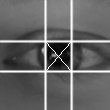
\includegraphics[scale=0.5]{img/pupil_section/EA_steps/EA_lines_intersection.png}}
        \hspace{8mm}
        \subfigure[Wykryte położenie źrenicy]{\label{fig:ea_pupil_detected}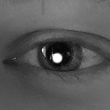
\includegraphics[scale=0.50]{img/pupil_section/EA_steps/EA_pupil_detected.png}}
    \end{center}
    \caption{Kolejne etapy wykrywania źrenic metodą EA}
    \label{fig:ea_steps}
\end{figure}
\newpage

\section{Landmarks} \label{section:landmarks}

Są to punkty nakładane na twarz wokół interesujących obszarów - takich jak oczy, nos czy usta. Pozwalają określić położenie, rozmiar czy kształt tych obiektów. Mogą być również użyte do predykcji czy mamy zamknięte/otwarte oczy lub czy się uśmiechamy. 

\subsection{OpenCV-contrib}
Dodatkowe moduł opencv facemark (\textit{OpenCV-contrib}) zawiera trzy algorytmy detekcji landmarków:

\begin{itemize}
    \item Kazemi
    \item AAM
    \item LBF
\end{itemize}

\subsubsection{FacemarkLBF}

Używając metody FacemarkLBF oraz modelu \textit{lbfmodel.yaml} określiłem punkty orientacyjne twarzy. \cite{landmarkSatyaMallick}

\begin{figure}[!h]
    \begin{center}
        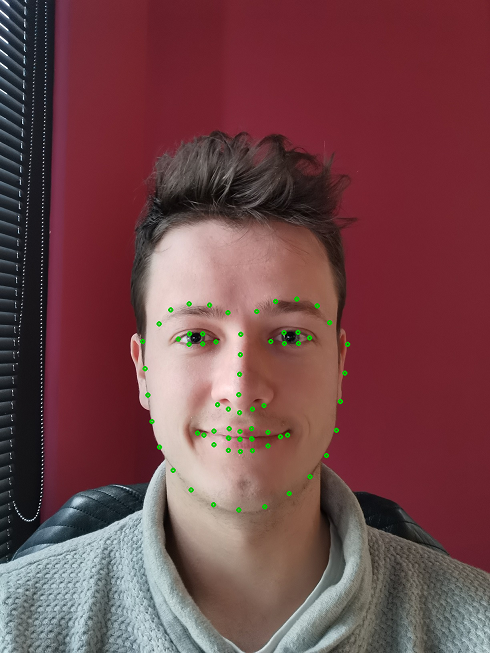
\includegraphics[scale=0.6]{img/landmark_section/landmarks_1.png}
        \caption{Twarz z naniesionymi landmarkami}
        \label{fig:landmarks_1}
    \end{center}
\end{figure}


\newpage

\section{EAR - Eye Aspect Ratio}
Metoda polegająca na obliczeniu \textit{EAR}  \cite{EARRaspberryPi} \cite{eyeBlinkEARRosebrock}, czyli stosunek otwarcia oczu - wysokość do szerokości widocznej części gałki ocznej. Wykorzystuje się tu landmarki (patrz rozdz. \hyperref[{section:landmarks}]{\textit{\ref{section:landmarks}.Landmarks}}) naniesione dookoła oczu.

\subsection{Wzór obliczania EAR}
Zależnie od ilości punktów wokół oka będzie różny wzór obliczania EAR.\\
Dla 6 punktów:
\begin{align}
    EAR = \frac{dist(L_0, L_1) + dist(L_2, L4)}{2 * dist(L_3, L_5)}
\end{align}
\\
Natomiast, dla 4 punktów:
\begin{align}
    EAR = \frac{dist(L_0, L_2)}{dist(L_1, L_3)}
\end{align}

Gdzie \textit{$L_x$} to kolejne landmarki dokoła oczu, a \textit{dist} to odległość między dwoma punktami (odległość euklidesowa).\\

\subsection{Zasada działania EAR w kontekście mrugania}

W teorii otwarte oczy będą miały większy wymiar liczbowy EAR, niż oczy zamknięte. Na \hyperref[{fig:theoretical_eye_landmarks}]{\textit{rysunku \ref{fig:theoretical_eye_landmarks}}} widać, że oko otwarte ma większe odległości między punktami pionowymi niż w przypadku  oka zamkniętego. Dzięki takim różnicą możemy wykryć spadek wskaźnika EAR poniżej pewnego ustalonego poziomu oznaczający zamknięcie oka, natomiast wzrost otwarcie oka. Całościowo obserwując zmiany np. za pomocą pochodnej jesteśmy w stanie stwierdzić mrugnięcie.

\begin{figure}[!h]
    \begin{center}
        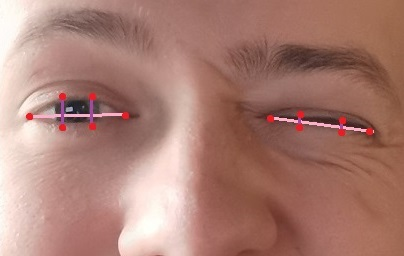
\includegraphics[scale=0.35]{img/landmark_section/theoretical_eye_landmarks.jpg}
        \caption{Teoretyczny rozmieszczene landmarków wokół oczu wraz z naniesionymi połączeniami do obliczenia EAR}
        \label{fig:theoretical_eye_landmarks}
    \end{center}
\end{figure}


\subsection{Testowanie z użyciem landmarków LBF opencv-contrib
}

\subsubsection{Test z użyciem kamery na żywo}

Wykonałem kilka krótkich testów z użyciem obrazu pochodzącego z przedniej kamery telefonu. 
\\
Poniżej znajdują się trzy testy, na których mrugnąłem tylko raz - lewym okiem, prawym i oboma na raz.

\begin{figure}[!h]
    \centering
    \begin{tikzpicture}
        \begin{axis}[
            xlabel = {Nr klatki obrazu z kamery},
            ylabel = {EAR},
            height = 0.5\linewidth,
            width = \linewidth,
            ymin= {0.10},
            ymax={0.30},
            ytick = {0.10, 0.12, 0.14, 0.16, 0.18, 0.20, 0.22, 0.24, 0.26, 0.28, 0.30},
            ymajorgrids = {true},
        ]
            \addplot[color=blue, mark=square*] table [x=x, y=a, col sep=comma] {csv/ear_left_1.csv};
            \addplot[color=red, mark=square*] table [x=x, y=b, col sep=comma] {csv/ear_left_1.csv};
        \end{axis}
    \end{tikzpicture}
    \caption{Mrugnięcie lewym okiem}
    \label{fig:left_eye_blink}
\end{figure}


\begin{figure}[!h]
    \centering
    \begin{tikzpicture}
        \begin{axis}[
            xlabel = {Nr klatki obrazu z kamery},
            ylabel = {EAR},
            height = 0.5\linewidth,
            width = \linewidth,
            ymin= {0.10},
            ymax={0.30},
            ytick = {0.10, 0.12, 0.14, 0.16, 0.18, 0.20, 0.22, 0.24, 0.26, 0.28, 0.30},
            ymajorgrids = {true},
        ]
            \addplot[color=blue, mark=square*] table [x=x, y=a, col sep=comma] {csv/ear_right_1.csv};
            \addplot[color=red, mark=square*] table [x=x, y=b, col sep=comma] {csv/ear_right_1.csv};
        \end{axis}
    \end{tikzpicture}
    \caption{Mrugnięcie prawym okiem}
    \label{fig:right_eye_blink}
\end{figure}

\begin{figure}[!h]
    \centering
    \begin{tikzpicture}
        \begin{axis}[
            xlabel = {Nr klatki obrazu z kamery},
            ylabel = {EAR},
            height = 0.5\linewidth,
            width = \linewidth,
            ymin= {0.10},
            ymax={0.30},
            ytick = {0.10, 0.12, 0.14, 0.16, 0.18, 0.20, 0.22, 0.24, 0.26, 0.28, 0.30},
            ymajorgrids = {true},
        ]
            \addplot[color=blue, mark=square*] table [x=x, y=a, col sep=comma] {csv/ear_both_1.csv};
            \addplot[color=red, mark=square*] table [x=x, y=b, col sep=comma] {csv/ear_both_1.csv};
        \end{axis}
    \end{tikzpicture}
    \caption{Mrugnięcie oboma oczami na raz}
    \label{fig:both_eyes_blink}
\end{figure}


Testy z pojedynczym mruganiem w krótkim okresie czasu dają przyzwoite wyniki i można na nich okreslić moment mrugania. W szczególności przy mrugnięciu jednym okiem.\\

Poniżej rozciągnąłem w czasie test na sekwencje kilku mrugnięć.

\begin{figure}[!h]
    \centering
    \begin{tikzpicture}
        \begin{axis}[
            xlabel = {Nr klatki obrazu z kamery},
            ylabel = {EAR},
            height = 0.5\linewidth,
            width = \linewidth,
            ymin= {0.10},
            ymax={0.30},
            ytick = {0.10, 0.12, 0.14, 0.16, 0.18, 0.20, 0.22, 0.24, 0.26, 0.28, 0.30},
            ymajorgrids = {true},
        ]
            \addplot[color=blue, mark=square*] table [x=x, y=a, col sep=comma] {csv/ear_long_1.csv};
            \addplot[color=red, mark=square*] table [x=x, y=b, col sep=comma] {csv/ear_long_1.csv};
        \end{axis}
    \end{tikzpicture}
    \caption{Kilka mrugnięć}
    \label{fig:multi_blinks_1}
\end{figure}

\begin{figure}[!h]
    \centering
    \begin{tikzpicture}
        \begin{axis}[
            xlabel = {Nr klatki obrazu z kamery},
            ylabel = {EAR},
            height = 0.5\linewidth,
            width = \linewidth,
            ymin= {0.10},
            ymax={0.30},
            ytick = {0.10, 0.12, 0.14, 0.16, 0.18, 0.20, 0.22, 0.24, 0.26, 0.28, 0.30},
            ymajorgrids = {true},
        ]
            \addplot[color=blue, mark=square*] table [x=x, y=a, col sep=comma] {csv/ear_long_2.csv};
            \addplot[color=red, mark=square*] table [x=x, y=b, col sep=comma] {csv/ear_long_2.csv};
        \end{axis}
    \end{tikzpicture}
    \caption{Kilka mrugnięć}
    \label{fig:multi_blinks_2}
\end{figure}

\begin{figure}[!h]
    \centering
    \begin{tikzpicture}
        \begin{axis}[
            xlabel = {Nr klatki obrazu z kamery},
            ylabel = {EAR},
            height = 0.5\linewidth,
            width = \linewidth,
            ymin= {0.10},
            ymax={0.30},
            ytick = {0.10, 0.12, 0.14, 0.16, 0.18, 0.20, 0.22, 0.24, 0.26, 0.28, 0.30},
            ymajorgrids = {true},
        ]
            \addplot[color=blue, mark=square*] table [x=x, y=a, col sep=comma] {csv/ear_long_3.csv};
            \addplot[color=red, mark=square*] table [x=x, y=b, col sep=comma] {csv/ear_long_3.csv};
        \end{axis}
    \end{tikzpicture}
    \caption{Kilka mrugnięć}
    \label{fig:multi_blinks_3}
\end{figure}

Tu również z dużym prawdopodobieństwem można okreśilć, w których klatkach wystąpiło mrugnięcie - widać gwałtowne obniżenie wartości EAR.
\\
Najlepsze wyniki były w przypadku pierwszego testu, ponieważ widać wtedy znaczną różnicę EAR między otwartym ($\sim0.26 - 0.30$), a zamkniętym okiem ($\sim0.12-0.18$). Na pozostałych testach różnice nie były już tak znaczące - na ostatnich dwóch wykresach otwarte i zamknięte oko ma niewielką różnicę w EAR. Takie małe różnice wyników mogą uniemożliwić prawidłową detekcję.

\vspace{3mm}
W każdym z przypadków testowych EAR dla jednego i drugiego oka prawie się pokrywają. Nawet przy mruganiu tylko jednym. Nie pozwoli to więc okręślić, którym okiem użytkownik mrugał.

\vspace{3mm}

Niewątpliwą trudnością w przypadku tej metody byłoby określenie progu wartości EAR, które zakwalifikowałbym jako mrugnięcie. Patrząc na wykresy powyżej można by przyjąć, że jest to wartość koło $~0.18$. Jednak w przypadku ostatecznego wyboru tej metody wymagałoby to dodatkowych badań celem określenia tej wartości.


\subsubsection{Niedokładność nakładania landmarków}

Patrząc jednak na położenie tych landmarków wokół oczu mam wątpliwości co do skuteczności tej metody:

\begin{figure}[!h]
    \begin{center}
        \subfigure[]{\label{fig:landmarks_accuracy_1}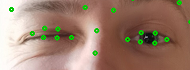
\includegraphics[scale=1.6]{img/landmark_section/landmarks_accuracy_1.png}}
        \hspace{8mm}
        \subfigure[]{\label{fig:landmarks_accuracy_2}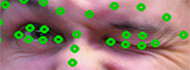
\includegraphics[scale=1.6]{img/landmark_section/landmarks_accuracy_2.png}}
    \end{center}
    \caption{Landmarki na oczach otwartych/zamkniętych}
    \label{fig:landmarks_accuracy_}
\end{figure}

Jak widać algorytm całkiem dobrze radzi sobie z rozmieszczeniem landmarków w przypadku otwartych oczu. Natomiast gdy oczy są zamknięte widać dużą niedokładność, która na pewno w dużym stopniu utrudnia prawidłową detekcję mrugnięcia.


%--------------------------------------------
% Literatura
%--------------------------------------------
\cleardoublepage % Zaczynamy od nieparzystej strony
\printbibliography

%--------------------------------------------
% Spisy (opcjonalne)
%--------------------------------------------
\newpage
\pagestyle{plain}

% Wykaz symboli i skrótów.
% Pamiętaj, żeby posortować symbole alfabetycznie
% we własnym zakresie. Ponieważ mało kto używa takiego wykazu,
% uznałem, że robienie automatycznie sortowanej listy
% na poziomie LaTeXa to za duży overkill.
% Makro \acronymlist generuje właściwy tytuł sekcji,
% w zależności od języka.
% Makro \acronym dodaje skrót/symbol do listy,
% zapewniając podstawowe formatowanie.
% //AB
\vspace{0.8cm}

\listoffigurestoc     % Spis rysunków.
\vspace{1cm}          % vertical space
\listoftablestoc      % Spis tabel.
\vspace{1cm}          % vertical space
\listofappendicestoc  % Spis załączników

% Załączniki
%\newpage
%\appendix{Nazwa załącznika 1}
%\lipsum[1-8]

%\newpage
%\appendix{Nazwa załącznika 2}
%\lipsum[1-4]

% Używając powyższych spisów jako szablonu,
% możesz tu dodać swój własny wykaz bądź listę,
% np. spis algorytmów.

\end{document} % Dobranoc.
